\subsection*{Q. 2}
\subsubsection*{Four-bit Parity Generator}
\vspace{-1.2em}
\begin{longtable}[c]{cccc|c}
\multicolumn{4}{l|}{Input 4-bit message} & \multicolumn{1}{l}{Odd parity generator} \\ \hline
\endfirsthead
%
\endhead
%
\hline
\endfoot
%
\endlastfoot
%
A        & B        & C        & D       & P                                        \\ \hline
0        & 0        & 0        & 0       & 1                                        \\
0        & 0        & 0        & 1       & 0                                        \\
0        & 0        & 1        & 0       & 0                                        \\
0        & 0        & 1        & 1       & 1                                        \\
0        & 1        & 0        & 0       & 0                                        \\
0        & 1        & 0        & 1       & 1                                        \\
0        & 1        & 1        & 0       & 1                                        \\
0        & 1        & 1        & 1       & 0                                        \\
1        & 0        & 0        & 0       & 0                                        \\
1        & 0        & 0        & 1       & 1                                        \\
1        & 0        & 1        & 0       & 1                                        \\
1        & 0        & 1        & 1       & 0                                        \\
1        & 1        & 0        & 0       & 1                                        \\
1        & 1        & 0        & 1       & 0                                        \\
1        & 1        & 1        & 0       & 0                                        \\
1        & 1        & 1        & 1       & 1                                        \\ \hline
\end{longtable}
\begin{center}
\begin{karnaugh-map}[4][4][1][$CD$][$AB$]
\minterms{0,3,5,6,9,10,12,15}
\implicant{0}{0}
\implicant{3}{3}
\implicant{5}{5}
\implicant{6}{6}
\implicant{9}{9}
\implicant{10}{10}
\implicant{12}{12}
\implicant{15}{15}
\end{karnaugh-map}
\end{center}
\vspace{-2.5em}
\begin{align*}
F(A,B,C,D)&=A'B'C'D'+A'B'CD+A'BC'D+A'BCD'+ABC'D'+ABCD+AB'C'D+AB'CD'\\
&=A'D'(BC+B'C')+A'D(B'C+BC')+AD'(BC'+B'C)+AD(BC+B'C')\\
&=A'D'(B\oplus C)'+A'D(B\oplus C)+AD'(B\oplus C)+AD(B\oplus C)'\\
&=(A'D'+AD)(B\oplus C)'+(A'D+AD')(B\oplus C)\\
&=(A\oplus D)'(B\oplus C)'+(A\oplus D)(B\oplus C)\\
&=((A\oplus D)\oplus (B\oplus C))'
\end{align*}
\centerline{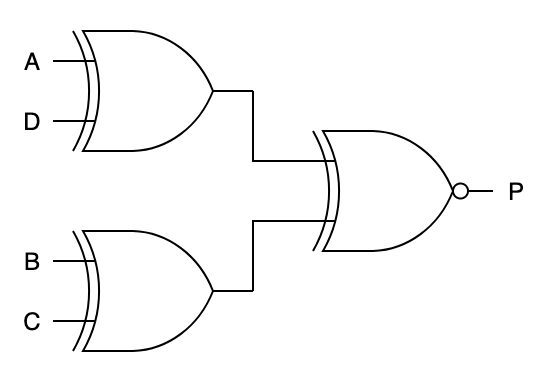
\includegraphics[width=0.4\textwidth]{fig/f21}}


\subsubsection*{Three-bit Parity Checker}
\vspace{-1.2em}
% Please add the following required packages to your document preamble:
% \usepackage{longtable}
% Note: It may be necessary to compile the document several times to get a multi-page table to line up properly
\begin{longtable}[c]{cccc|c}
\multicolumn{4}{l|}{Input (3+1)-bit} & \multicolumn{1}{l}{Odd parity checker} \\ \hline
\endfirsthead
%
\endhead
%
\hline
\endfoot
%
\endlastfoot
%
A       & B       & C       & P      & $C_P$                                   \\ \hline
0       & 0       & 0       & 0      & 1                                      \\
0       & 0       & 0       & 1      & 0                                      \\
0       & 0       & 1       & 0      & 0                                      \\
0       & 0       & 1       & 1      & 1                                      \\
0       & 1       & 0       & 0      & 0                                      \\
0       & 1       & 0       & 1      & 1                                      \\
0       & 1       & 1       & 0      & 1                                      \\
0       & 1       & 1       & 1      & 0                                      \\
1       & 0       & 0       & 0      & 0                                      \\
1       & 0       & 0       & 1      & 1                                      \\
1       & 0       & 1       & 0      & 1                                      \\
1       & 0       & 1       & 1      & 0                                      \\
1       & 1       & 0       & 0      & 1                                      \\
1       & 1       & 0       & 1      & 0                                      \\
1       & 1       & 1       & 0      & 0                                      \\
1       & 1       & 1       & 1      & 1                                      \\ \hline
\end{longtable}
\begin{center}
\begin{karnaugh-map}[4][4][1][$CP$][$AB$]
\minterms{0,3,5,6,9,10,12,15}
\implicant{0}{0}
\implicant{3}{3}
\implicant{5}{5}
\implicant{6}{6}
\implicant{9}{9}
\implicant{10}{10}
\implicant{12}{12}
\implicant{15}{15}
\end{karnaugh-map}
\end{center}
\vspace{-2.5em}
\begin{align*}
F(A,B,C,P)&=A'B'C'P'+A'B'CP+A'BC'P+A'BCP'+ABC'P'+ABCP+AB'C'P+AB'CP'\\
&=A'P'(BC+B'C')+A'P(B'C+BC')+AP'(BC'+B'C)+AP(BC+B'C')\\
&=A'P'(B\oplus C)'+A'P(B\oplus C)+AP'(B\oplus C)+AP(B\oplus C)'\\
&=(A'P'+AP)(B\oplus C)'+(A'P+AP')(B\oplus C)\\
&=(A\oplus P)'(B\oplus C)'+(A\oplus P)(B\oplus C)\\
&=((A\oplus P)\oplus (B\oplus C))'
\end{align*}
\centerline{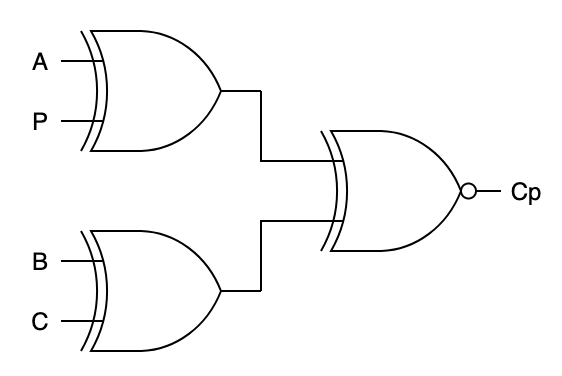
\includegraphics[width=0.4\textwidth]{fig/f22}}
